\documentclass[letterpaper]{article}
\usepackage{underscore}
\usepackage[left=2.0cm, right=2.0cm, top=2.0cm]{geometry}
\usepackage[utf8]{inputenc}
\usepackage{graphicx}
\usepackage{graphics}
\usepackage[spanish]{babel}
\usepackage{lipsum}
\usepackage{float}
\usepackage{subfigure}
\usepackage{biblatex}
\usepackage{csquotes}
\usepackage{color}
\title{\textbf{Brazo Programable de Fácil Uso }} 

%plantillas de comandos 
%subrrayado con color de texto    \colorbox{blue}{\textcolor{white}{caca de la vaxa}}
\author{Ledesma Hernández Miguel Ángel, Carrasco Quiñones Karla Daniela, Reyna Gurrola Marcela\\ y Alcantar Díaz Joel Alejandro.}
\date{08/11/2019}
\begin{document}
\maketitle
\begin{center}
    
\includegraphics[scale=0.5]{Img/UPZMGlog.png}\\
    \vspace{1cm}
    Universidad Politécnica de la Zona Metropolitana de Guadalajara.\\
    \vspace{1cm}
Ing. en Mecatrónica.
\end{center}\newpage
\begin{large}
    \begin{LARGE}
        \textbf{Planteamiento del problema.}\\
    \end{LARGE}%hola bebé
    \begin{large}
    En la actualidad las máquinas de índole robótica están presentes en varias empresa que poseen un sistema automatizado a pesar de la complejidad en la programación de estos, lo cual lleva a muchas empresas emergentes e incluso ya consolidas a no poder hacer uso de estos equipos por la complejidad que conlleva la programación de un equipo de estos y el temor de que no cualquiera puede usarlas correctamente por falta de personal capacitado para operar las mismas en la empresa. Esto genera que se requiera contratar un programador experto, ya que no se aprovecha al máximo funcionamiento de la maquinaria.\\
    Por lo que la complicación de no poder usarlo es por la necesidad de programar el equipo para poder ponerlo en marcha y generar ingresos. Esto es más que nada debido a la poca importancia que se le da en México al automatizar una fábrica, ya que se tiene que invertir mucho para instalar y acondicionar una máquina nueva en la empresa.\\
    Por esta razón es que una unidad que se pueda programar solamente moviendo un modelo similar a escala humana podría sustituir la programación en muchos casos y facilitar el uso de estas máquinas complejas y sofisticadas.\\
    \end{large}
\end{large}

\begin{large}
    \begin{LARGE}
       \textbf{Formular el problema.}\\
    \end{LARGE}
    ¿Es complicado utilizar una de estas máquinas?\\
    ¿Cuál es el nivel de programación que se necesita para programar una máquina robótica?\\
    ¿Quiénes pueden utilizarla?\\
    ¿Cuál es la mejor forma para programar y diseñar un GIU?\\
    
\end{large}

\begin{large}
    \begin{LARGE}
        \textbf{Objetivo general.}\\
    \end{LARGE}
     Crear un brazo mecánico con la capacidad de reflejar los movimientos del usuario mediante un guante. 
  
\end{large}

\begin{large}
    \begin{LARGE}
        \textbf{Objetivos del proyecto.}\\
    \end{LARGE}
    \begin{enumerate} 
        \item \colorbox{cyan}{Identificar los componentes necesarios para la contracción del brazo a escala.} 
        \item Programar una GIU .
        \item Generar una estructura de soporte para el brazo.
        \item Determinar los grados de movimiento del brazo.
        \item \colorbox{cyan}{Iniciar el armado del primer prototipo.}
        \item Idear un marco de pruebas para el prototipo.
        \item \colorbox{cyan}{Crear una fuente conmutada especialmente para el brazo.}
        \item Calcular los pesos y fuerzas de los motores a utilizar.
        \item \colorbox{cyan}{Crear PCB específicas para el brazo}
    \end{enumerate}
    %no escuho si me neeitan me escriben abajo de obj generales para escribir bien xd
\end{large}
\vspace{1.5cm}
\begin{large}
    \begin{LARGE}
        \textbf{Justificación.}\\
    \end{LARGE}
    %aquí tienes que poner el texto de la justificación
    % usa este comando si quieres poner un texto remarcado en azúl \colorbox{blue}{\textcolor{white}{caca de la vaxa}}
Este proyecto permitirá programar los movimientos del brazo robótico mediante una técnica espejo, lo cual evita es uso de comandos y fallas al momento de compilar el programa. Además de que cualquier persona que cuente con los conocimientos básicos sobre cómo guardar los movimientos del robot podrá usarlo y programarlo para cualquier cosa que desee. 
\end{large}
\vspace{1.8cm}\\
\begin{large}
    \begin{LARGE}
        \textbf{Delimitación.}\\
    \end{LARGE}
  Solo podrá moverse como demostración de las capacidades de lectura de los sensores, también una limitante es el material ya que sera construido con MDF y el control que puede tener el usuario. Además de contar con unas medidas de 40cm de ancho, 40cm de largo y 50cm de alto aproximadamente con el brazo completamente estirado.\\\\
  La principal limitante es económica por el bajo presupuesto que se le inyecta al proyecto, por esta razón se trata solo de un prototipo funcional.
\end{large}

\begin{large}
    \begin{LARGE}
        \textbf{Matriz de roles.}\\
        
    \end{LARGE}
    

%\begin{table}[]
\begin{tabular}{|c|c|c|c|c|}
\hline
    Actividades                         & Joel & Miguel & Marcela & Karla       \\ \hline
    Investigar sobre el desarrollo y    & Sí   &  Sí    &      Sí &  Sí         \\   
    en que nos puede ayudar             &      &        &         &             \\ \hline
    Cotizar el costo de los materiales  & Sí   &     Sí &     Sí  & No          \\
    requeridos para la realización del  &      &        &         &             \\
    brazo                               &      &        &         &             \\\hline
    Comprar los componentes requeridos  &   Sí & Sí     &   Sí    & No          \\
    para la realización del brazo.      &      &        &         &             \\ \hline
    Realizar el primer prototipo.       & Sí   & Sí     & Sí      & Sí          \\\hline
    Hacer pruebas con el brazo          & Sí   &Sí      & Sí      & Sí           \\
    para tener en cuenta los errores.   &      &        &         &             \\\hline
    Hacer reparaciones del brazo.       & Sí   & Sí     & Sí      & Sí           \\\hline
    Hacer la fuente de conmutada & Sí & No & Sí & No
      \\\hline
    Hacer las PCBs del circuito & No  & Sí  &  No &  Sí
       \\\hline
\end{tabular}
\end{large}\\ \newpage

 
   
   
   \begin{LARGE}
   \begin{figure}[htbp]
        \textbf{Diagrama de GANTT.}\\
       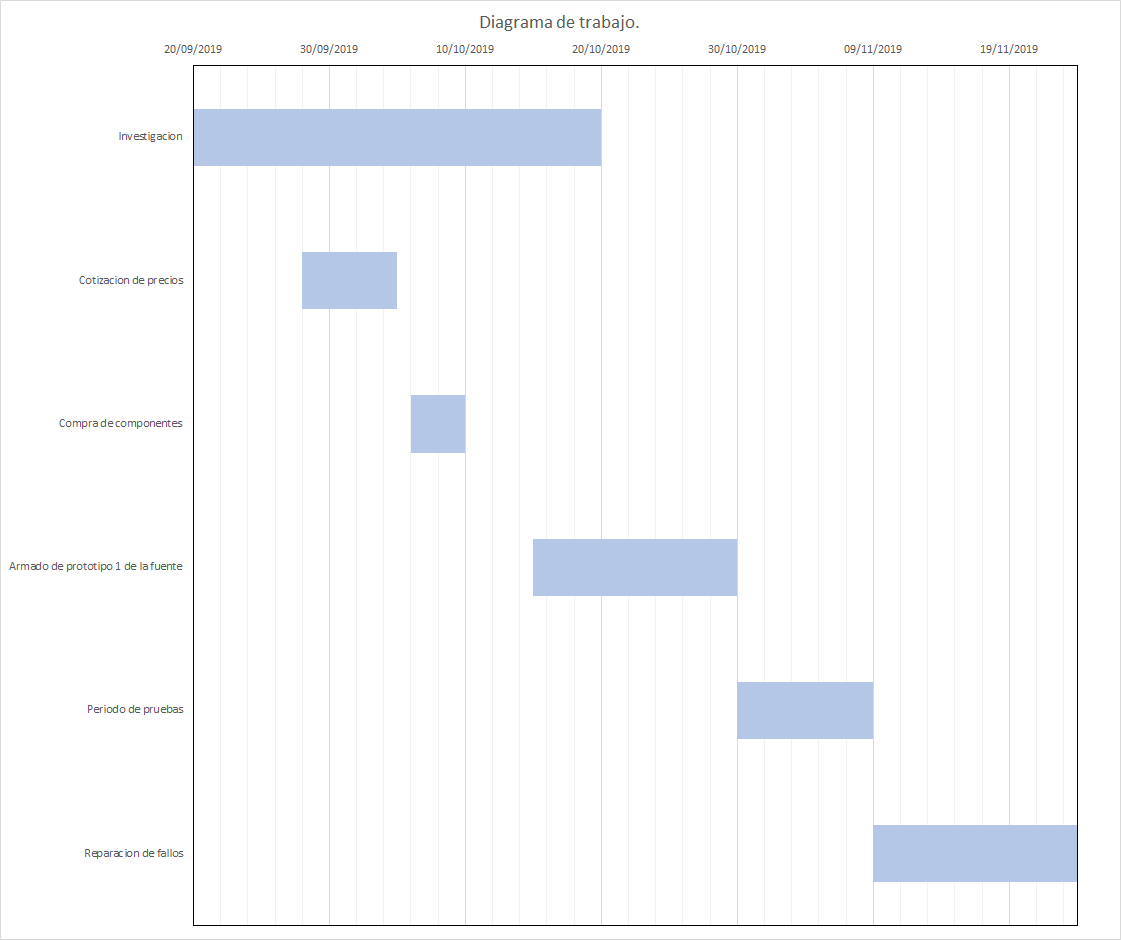
\includegraphics[width=17cm]{Img/gantt.png}
 \end{figure}
   \end{LARGE}
   \newpage
   \begin{large}
       \begin{large}
       \textbf{Matríz de materiales y costos.}
           \begin{table}[htbp]
\begin{tabular}{|l|l|l|l|} 
\hline
Producto      & Costos         & Modelo               & Descripción                            \\ \hline
Motor a pasos & 50 pesos       & 28byj-48             & Un motor programable                   \\ \hline
Raspberry     & 780 pesos      & pi 3 B+              & Una pequeña computadora tamaño tarjeta \\ \hline
Cables varios & 50c c/u        & cupper               & Utilidad de conexión                  \\ \hline
Resistencias  & 50c c/u        & Null                 & Resistores para controlar el flujo de corriente  \\ \hline
Impresión 3d  & X pesos        & Null                 & Impresiones varias                     \\ \hline
Tubos PVC     & 30 pesos metro & 1/2                  & Soportes del brazo                     \\ \hline
Estaño/cautín & 150 pesos      & generico             & Para soldar                            \\ \hline
Placa de base & X pesos        & depende del material & Donde se montará                       \\ \hline
Buzzer        & 25 pesos       & Null                 & Para el sonido                         \\ \hline
Leds          & 10 pesos c/u   & Null                 & Estilizar el modelo                    \\ \hline
Giroscopio    & 50 Pesos       & MPU6050              & Modulo de giroscopio y acelerómetro    \\ \hline
Potenciometro & 6 pesos c/u    & Null                 & Resistencia variable de 10k            \\ \hline
\end{tabular}
\end{table}
       \end{large}
   \end{large}
\\\\
\begin{large}
\textbf{Funcionamiento teorico.}\\\\
El brazo funciona a travez de la captación de movimientos en un sistema controlado por una mano humana. Este captará los movimientos para después traducirlos y enviarlos, el proceso cuenta de variables con mismos valores actualizandose constantemente con el valor de el anterior, como ejemplo de esto se encuentra u y $u'$, donde u=5 y $u'$=10, dentro de un código programado no se debe poner el caracter reservado de $" ' "$ pero se pone un identificador para el captador y para el emisor, dentro de este programa se hará el proceso de captación de u para después traducir y mandar señales a $u'$ teniendo como base un registro guardado de sus coordenadas relativas y/o absolutas dentro de un plano cartesiano lógico ubicado sobre el sistema. \\
Tomará cada motor como un sistema individual que en conjución con los demás hará un sistema complejo de agarre de pinza y movimiento. El agarre de pinza constará de dos estados, uno en el que la mano del usuario esté abierta(Estado1) y una donde la mano esté cerrada(Estado0), siendo posible escalar el proyecto para la detección exacta de la posición, reduciendo de dos estados a uno que traduzca la posición real del servomotor del usuario para replicar lo mismo en el sistema.
\\
\end{large}
\newpage
\begin{large}
\textbf{Explicación de la aportación  de cada materia cursada en el cuatrimestre al proyecto}


\begin{table}[htbp]
    \centering
   
   
    \begin{tabular}{|l|l|}
    \hline
Materias de 4to  &  Detalles de aportación al proyecto 
                        \\ \hline
Inglés & El inglés es necesario para programar y\\
        & leer la gran mayoría de información\\
        & disponible en internet.
                        \\ \hline
Ética profesional &  Es necesaria para determinar si estamos robando o no información\\
                  &  Tener una idea de las necesidades de las personas y poder empatizar\\
                  &  para poder crear un sistema que ayude a los usuarios
                  
                        \\\hline
Estructura y propiedades de los materiales & La selección de un material\\
                                 & resistente pero flexible como la\\
                                 & madera, además del tipo de adhesivo\\
                                 & que se utilizará.
                        \\\hline
Programación de periféricos & Para que el brazo se capaz de guardar\\
                            & los movimientos se necesita programarlo\\
                            & para lograr crear un interfaz más\\
                            & gráfica y amigable con el usuario.
                        \\\hline
Sistemas electrónicos de interfaz & La fuente que alimentará el brazo\\
                                 & deberá contar con los valores de\\
                                 & voltaje y corriente necesarios para\\
                                 & mantenerlo en óptimo funcionamiento.
                        \\\hline
Controladores lógicos programables & El funcionamiento principal del\\
                                &brazo se llevará a cabo gracias a una\\
                                & tarjeta que mediará los grados de\\
                                & movimiento del los servo-motores.\\
                                \hline
        
    \end{tabular}
\end{table}

\end{large}
\newpage
\begin{large}
    \textbf{Boceto preliminar}
             \begin{figure}[htbp]
                \centering
                \subfigure[Modelado preliminar]{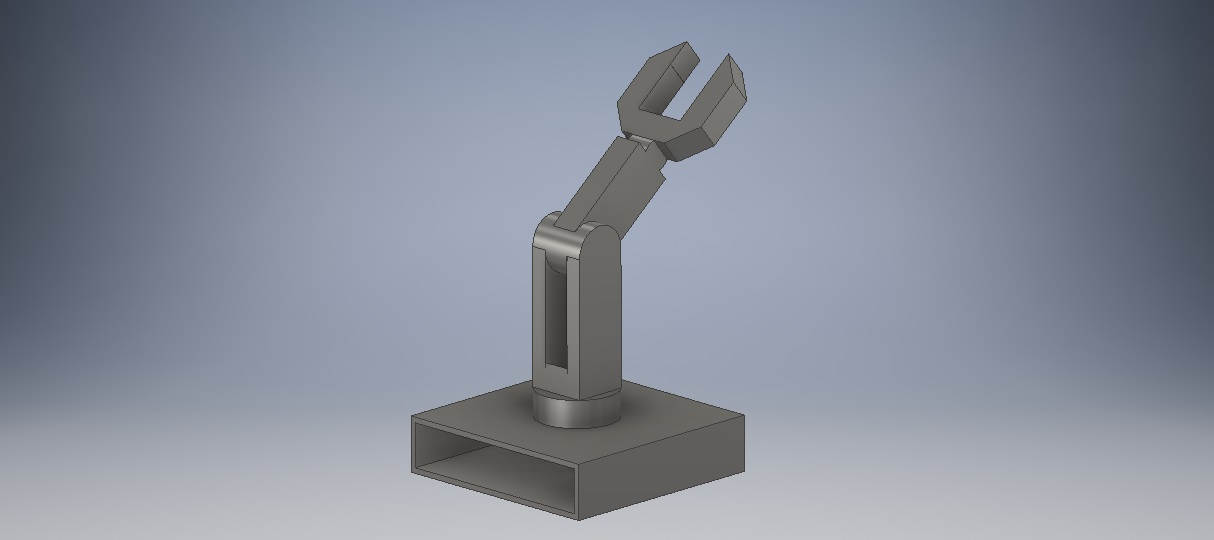
\includegraphics[scale=0.4]{Img/Brazo.jpg}}
                \subfigure[Medidas aproximadas y dibujo en mm]{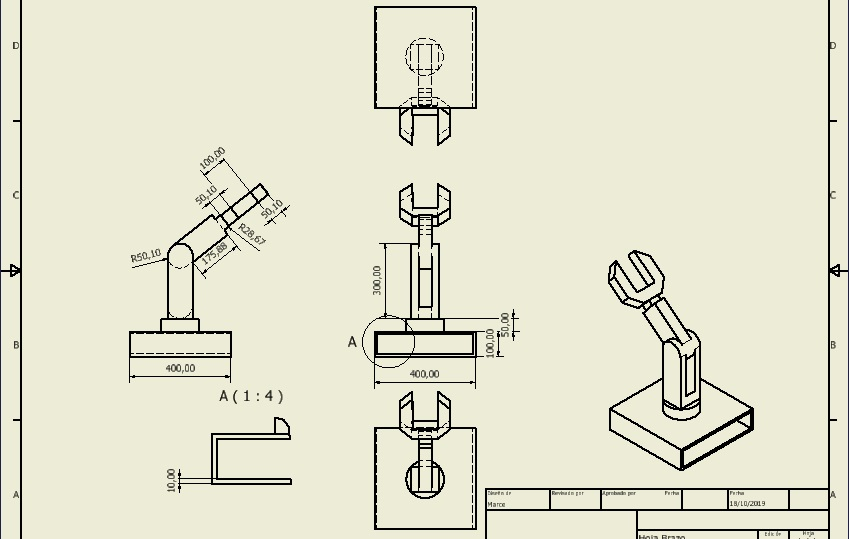
\includegraphics[scale=0.6]{Img/Hojabrazo.jpg}}
                \caption{Primer boceto del brazo}
                \label{fig:bra}
            \end{figure}
        \begin{LARGE}
    \end{LARGE}
\end{large}
 Nota: las medidas mostradas se encuentran en milímetros.\\
 
\newpage
    \begin{thebibliography}{x}
        \bibitem{MotPas} \textsc{Anónimo} \textit{"Motor a paso."} Recuperado de:\\ 
        https://www.polibits.gelbukh.com/2005\_32/Polibits\_32\_2005.pdf\#page=28
        \bibitem{FueCon} \textsc{Fuentes conmutadas.} Recuperado de:\\
        $https://www.electronicafacil.net/tutoriales/Fuentes-conmutadas.html$
        \bibitem{Fuente} \textsc{CAMERO, Alfonso Darío López; Elianny Treto and Crispí, Alberto Taboada} \textit{DISEÑO DE FUENTES CONMUTADAS.}Recuperado de:\\ //www.sciencedirect.com/science/article/pii/S1697791208701225 
        \bibitem{ComFuente} \textsc{Electrocomponentes, S. A.} \textit{Fuentes de alimentación.} (2012). Recuperado de:\\ https://sistemamid.com/panel/uploads/biblioteca/1/349/1259/6572/6603/78232.pdf 
\end{thebibliography}
\end{document}






